\section{Validation}

\subsection{Validation Methodology}

I validated each mechanism with small directed RISC-V programs run in
syscall-emulation mode, usually comparing a run with the feature
turned off against a run with it turned on. Python checkers then read
the program output, the committed instruction trace, the simulator
trace, and the statistics. They check that predictions, bypasses,
dependency handling, and recovery behave as intended. I wrote these
checkers alongside the implementation, so a passing result shows that
the behavior matches the design in the tested cases.

\subsection{Standalone LVP Validation}

The LVP suite has six test modes, and all 772 of its checks passed.
Each workload runs in four configurations: LVP off (A), prediction
only (B), prediction with dependent-load speculation (C), and C with
detailed tracing (CL). Configuration B separates training and lookup
from speculative use, and CL lets the checker follow each
producer-consumer pair. The committed instruction traces of A, B, and
C match for every workload.

\subsubsection{Workloads and Checks}

The main mode uses five directed workloads: Stable (constant values),
Phase (values that change, causing mispredictions), Fan-out (several
consumers of one prediction), Fault (memory faults on speculative
consumers), and Chain (a consumer that is itself a predicted
producer). It checks that predictions respect the confidence threshold
and PC window, and that speculative loads are issued only in
configuration C. All five workloads passed, with 473 checks.

The other five modes passed 299 checks. They cover confidence
thresholds of 1, 2, and 3, the PC window, rejection of invalid
configurations, counter updates, and table aliasing. For example, the
confidence test shows that a mismatch moves a saturated counter from
3 to 2 rather than resetting it. The alias test shows that PCs 2,048
bytes apart share an entry in the default 1,024-entry table.

\subsubsection{Recovery Checks}

The detailed traces recorded 255, 255, 32, and 26 recovery redirects
for Phase, Fan-out, Fault, and Chain. Every used wrong prediction causes exactly one redirect. No
redirect happens without an accepted consumer. Events occur in this
order:
\[
    \text{accept}
    <
    \text{validation}
    \leq
    \text{redirect}
    <
    \text{consumer squash}.
\]
It also checks that every committed speculative load used a correct
prediction, that affected consumers are discarded rather than
committed, and that the Fetch2 branch-predictor cleanup happens once
per redirect.

\subsection{ASTRA and V-ASTRA Validation}
\label{subsec:astra-vastra-validation}

ASTRA and V-ASTRA were tested in layers. Component tests cover the
predictor, the value cache, candidate selection, and older-store
conflicts. The tests then check that bypassed loads really
skip memory. These two kinds of tests are kept apart, because a
correct candidate does not guarantee that a load will bypass memory
or commit correctly.

\subsubsection{ASTRA Predictor}
\label{subsubsec:astra-validation}

The first ASTRA suite compares ASTRA turned off, ASTRA in shadow mode,
and shadow mode with detailed logging. Over ten loads in seven
functions, it recorded 640 committed loads and passed 78 checks. The
checker replays every logged lookup and update against a reference
model of the predictor. This covers indexing, stride calculation,
table updates, and retirement-order training. A second, targeted suite
passed 340 checks across seven modes. These cover cold prediction,
aliasing in both tables, destructive conflicts, wrong-path and fault
handling, invalid configurations, and running alongside LVP.

\subsubsection{Value Cache}
\label{subsubsec:vcache-validation}

The value-cache suite passed 157 checks in four modes: operations
(32), squash (34), fault (31), and non-interference (60). The
operations mode runs a 52-step sequence of loads, stores, and special
accesses, and replays the observed cache behavior against a reference
model. The squash and fault modes check that discarded or faulting
operations never update the cache. The non-interference mode compares
runs with the cache off and in shadow mode, including cycle counts.
It also checks that no diagnostic hit returns wrong data, and it found
none in 16,382 hits.

\subsubsection{V-ASTRA Candidates and Strict Verification}
\label{subsubsec:vastra-candidate-validation}

The V-ASTRA suite passed 276 checks covering candidate selection,
older-store conflicts, discarded and faulting loads, and
non-interference. With strict verification on and bypass off, 5,605
candidates had their value-cache data compared against real memory,
with no mismatches. This shows that the candidate data is correct. It
does not show that the bypass itself works, which is tested
separately below.

A negative control shows that the older-store scan is needed. With the
scan on, 14 conflicting loads were rejected and no wrong data was
seen. With the scan turned off through a test-only option, six
candidates held stale data from older stores still in flight. With
strict verification also on, that run stopped with the expected error,
because the base was correct but the data was not.

\subsubsection{Load Bypass}
\label{subsubsec:vastra-bypass-validation}

The bypass suite compares runs with bypass off and on. It checks the
program output, the committed trace, memory-access traces, and bypass
statistics. It passed 297 checks across 17 modes, covering store and
atomic conflicts, discarded and faulting loads, fallbacks, split and
special accesses, system calls, LVP coexistence, and configuration
rules. In one mode, 22 bypassed loads completed without any memory
request, and data-cache read accesses dropped by exactly 22.

\subsection{Dependency Handling Validation}
\label{subsec:dependency-handling-validation}

These tests first measure how MinorCPU handles dependents under
stall-on-use timing, and then check the two designs of
Section~\ref{sec:impl-sb}. Design~A only lets a dependent issue
earlier. Design~B also gives a dependent load the value it needs to
send its memory request.

\subsubsection{Stall-on-Use Baseline}
\label{subsubsec:stall-on-use-validation}

The stall-on-use configuration is the baseline configuration with
\texttt{extraAssumedLat} set from 2 to 0, and no value predictor. Its
workload has two timing scenarios, each run 12 times. The first puts
independent instructions between a long-latency load and its
dependent. The second uses an older cache-missing load to delay the
producer's commit after its data has already arrived, which separates
data arrival from dependency release.

The suite passed 17 checks. With default timing, the dependent issues
two cycles after the producer issues. Under stall-on-use, it issues
exactly when the producer commits
(\(D_{\mathrm{issue}}-L_{\mathrm{commit}}=0\)), even in the second
scenario, where the data arrived at least 106 cycles earlier.
Independent instructions can still issue before the producer commits.
In this MinorCPU setup, then, a dependency is released at commit, not
when the data arrives.

\subsubsection{Design~A: Scoreboard Release}
\label{subsubsec:scoreboard-release-validation}

Design~A was tested by comparing runs with release off and on under
stall-on-use timing, and passed 255 checks. The tests confirm that
each release happens exactly once and only after a successful bypass,
that released loads send no memory request, and that the scoreboard
stays consistent through commit, squash, fault, drain, and statistics
reset. Directed cases cover successful bypasses, base mismatches,
value-cache misses, and older-store conflicts.

In the successful case, the dependent issues within two cycles of the
release and at least 50 cycles before the producer commits, but it
still commits after the producer. The gap between the two commits
shrinks from three cycles to one. However, both runs take exactly
215,697 cycles. In this workload, Design~A lets the dependent start
earlier without reducing total runtime.

\subsubsection{Design~B: Validated-Value Forwarding}
\label{subsubsec:validated-value-forwarding-validation}

Design~B was tested by comparing runs with forwarding off and on, and
passed 275 checks from its configuration, directed, and lifecycle
tests. The directed tests checked 96 forwarded values against the
producers' committed values, with no mismatches. They recorded 108
admitted consumers, of which 96 committed and 12 were squashed. The
tests also checked addresses, producer-consumer ordering, the
\texttt{Pending} and \texttt{Failed} states, and wrong-path cleanup.
With forwarding off, dependent requests wait for the producer to
commit.

\subsection{META Integration and Recovery Validation}
\label{subsec:meta-integration-recovery-validation}

These tests check META as a whole: its configuration rules, which
source it picks, its bookkeeping, recovery from wrong LVP predictions
that were used, and the provisional-base modes.

\subsubsection{Configuration and Source Selection}
\label{subsubsec:meta-configuration-directed-tests}
\label{subsubsec:meta-lifecycle-source-selection}

Three META suites passed: 25 configuration checks, 281 directed
checks, and 4,625 lifecycle checks. They cover valid and invalid
configurations, interactions between the predictors, recovery, and
producer-consumer bookkeeping. The directed checker also checks every
recorded META decision against the selection rules of
Section~\ref{sec:impl-meta}. Two more META suites are there i.e. the ASTRA--LVP experiments behind Sections~\ref{subsubsec:meta-provisional-bases-validation}
and~\ref{subsubsec:meta-forced-misprediction-recovery}, and the
alignment regression of Section~\ref{subsubsec:meta-alignment-retry}.

All four outcomes of those rules occurred in the tests: V-ASTRA
selected, a wait for a pending V-ASTRA record, LVP used after
V-ASTRA failed, and no prediction. Some V-ASTRA-served loads also had their own LVP predictions, but
those predictions could not be used at that point. In the forwarding
workload, every V-ASTRA-served load either committed or was squashed.

\subsubsection{Provisional ASTRA Bases from LVP Predictions}
\label{subsubsec:meta-provisional-bases-validation}

The three modes of Section~\ref{sec:impl-provisional} were tested on
two workloads. In the random-base workload, the LVP predictions used
as bases are always correct. In the forced-misprediction workload,
some of them are wrong.
Figure~\ref{tab:meta-provisional-results} shows the results. The
created, validated, and dropped counts come from the measured region,
while the LVP-served-load and candidate counts cover the whole run.

\begin{figure}[H]
    \centering
    \pgfplotsset{
        provbar/.style={
            ybar,
            width=\linewidth,
            height=3.7cm,
            ymin=0,
            enlarge x limits=0.11,
            symbolic x coords={RBoff,RBtrain,RBcand,FMtrain,FMcand},
            xtick=data,
            xticklabels={{Random base\\off},{Random base\\train},
                         {Random base\\candidate},{Forced mispred.\\train},
                         {Forced mispred.\\candidate}},
            xticklabel style={align=center, font=\footnotesize},
            yticklabel style={font=\footnotesize},
            ylabel style={font=\footnotesize},
            legend style={at={(0.5,1.03)}, anchor=south,
                          legend columns=-1, font=\footnotesize,
                          draw=none},
            nodes near coords,
            every node near coord/.append style={font=\tiny, rotate=90, anchor=west},
            ymajorgrids,
            grid style={gray!25},
        }
    }

    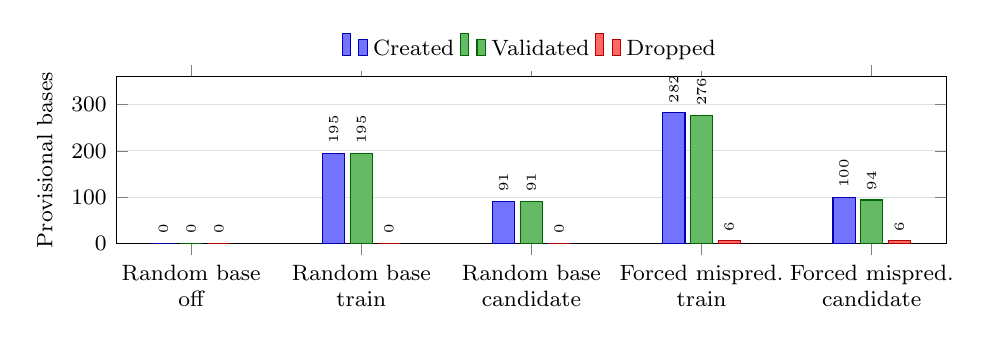
\begin{tikzpicture}
    \begin{axis}[provbar, bar width=8pt, ymax=360,
                 ylabel={Provisional bases}]
        \addplot[fill=blue!55, draw=blue!70!black] coordinates
            {(RBoff,0) (RBtrain,195) (RBcand,91) (FMtrain,282) (FMcand,100)};
        \addplot[fill=green!55!black!60, draw=green!40!black] coordinates
            {(RBoff,0) (RBtrain,195) (RBcand,91) (FMtrain,276) (FMcand,94)};
        \addplot[fill=red!60, draw=red!70!black] coordinates
            {(RBoff,0) (RBtrain,0) (RBcand,0) (FMtrain,6) (FMcand,6)};
        \legend{Created, Validated, Dropped}
    \end{axis}
    \end{tikzpicture}

    \vspace{0.2em}

    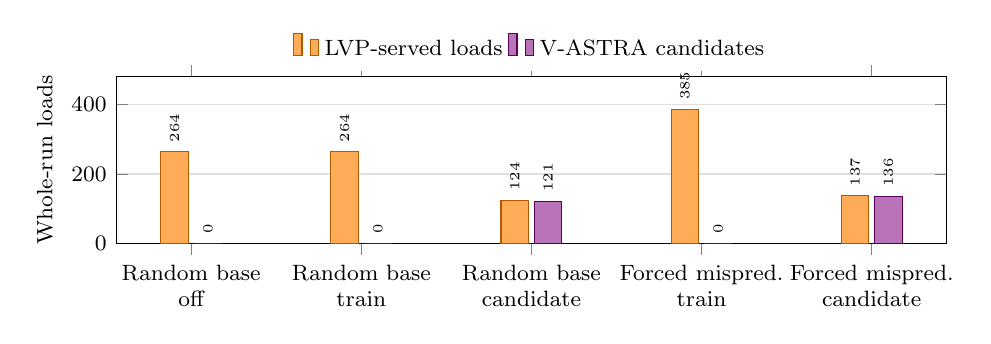
\begin{tikzpicture}
    \begin{axis}[provbar, bar width=10pt, ymax=480,
                 ylabel={Whole-run loads}]
        \addplot[fill=orange!65, draw=orange!70!black] coordinates
            {(RBoff,264) (RBtrain,264) (RBcand,124) (FMtrain,385) (FMcand,137)};
        \addplot[fill=violet!55, draw=violet!70!black] coordinates
            {(RBoff,0) (RBtrain,0) (RBcand,121) (FMtrain,0) (FMcand,136)};
        \legend{LVP-served loads, V-ASTRA candidates}
    \end{axis}
    \end{tikzpicture}

    \caption{Provisional-base results. Top: provisional bases
    created, validated, and dropped. Bottom: LVP-served loads
    and the V-ASTRA candidates formed from them over the whole run
    (candidacy does not apply in \texttt{off} mode).}
    \label{tab:meta-provisional-results}
\end{figure}

The \texttt{train} mode never turned a provisional base into a V-ASTRA
candidate, while \texttt{candidate} mode did, as intended. No
provisional load created a forwarding record in any mode. In the
random-base \texttt{candidate} run, every candidate's predicted base
matched the LVP value. In the forced-misprediction \texttt{candidate}
run, eight loads bypassed memory before their LVP value was
validated. When the wrong prediction was detected, all eight were
discarded. So correctness comes from the later validation and
recovery, not from validating the base before it is used.

\subsubsection{Forced Misprediction and Recovery Ordering}
\label{subsubsec:meta-forced-misprediction-recovery}

Under META, a wrong LVP prediction should cause recovery only if a
load actually used it (Section~\ref{sec:impl-meta}). Four directed
cases test this:
\begin{itemize}
    \item \textbf{Wrong value used:} three recoveries occurred, the
    same as in the LVP-only control.
    \item \textbf{Wrong value not used:} three wrong predictions
    caused no recovery, while the LVP-only control recovered three
    times.
    \item \textbf{V-ASTRA consumers:} three wrong LVP predictions
    caused no LVP recovery, because four loads used V-ASTRA values
    instead.
    \item \textbf{Forced misprediction:} nine wrong predictions were
    used, each caused one redirect, and every affected load was
    discarded before commit.
\end{itemize}

In the forced-misprediction case, the trace shows nine redirects over
the whole run, while the statistics show six recoveries in the
measured region. The two numbers cover different parts of the run.
The same nine recoveries happened in \texttt{off}, \texttt{train}, and
\texttt{candidate} modes. In \texttt{candidate} mode, the trace also
confirmed the bypass, validation, redirect, and discard order of
Section~\ref{sec:impl-provisional} for all eight early bypasses.

\subsubsection{Alignment and Provisional-State Retry Regression}
\label{subsubsec:meta-alignment-retry}

This test targets the bug described in
Section~\ref{sec:impl-provisional}. Before the fix, it reproduced the
failure where an LVP-fed load with a provisional base hit an alignment
fault before entering the LSQ, ran again, and reached commit with a
stale provisional base.

After the fix, the test passed all 92 checks in four configurations:
no prediction, and META in \texttt{off}, \texttt{train}, and
\texttt{candidate} modes. It recorded 60 provisional bases created and
60 dropped, one for each of the 60 early alignment faults. Each
faulting attempt was followed by exactly one re-execution, with no
architectural faults and no training on a misaligned base. The output
and committed values matched the no-prediction run over 2,611
instructions.

\subsection{Final Regression}
\label{subsec:final-regression}

After the last source changes, every suite in this section was rerun
together on the final source revision. This covered the ASTRA,
value-cache, V-ASTRA, standalone LVP, load-bypass, stall-on-use,
Design~A, Design~B, and drain and statistics-reset suites, and all
five META suites. Every suite passed with no failures, and the check
counts matched those reported above, except in two suites. The META
lifecycle and ASTRA--LVP suites ran 60 and 216 more checks,
respectively. These extra checks all come from two drain and
statistics-reset workloads that produced more statistics windows, and
each window adds its own set of checks. They also all passed.
